\ifx\wholebook\relax \else
% ------------------------

\documentclass[b5paper]{ctexart}
\usepackage[nomarginpar
  %, margin=.5in
]{geometry}

\addtolength{\oddsidemargin}{-0.05in}
\addtolength{\evensidemargin}{-0.05in}
\addtolength{\textwidth}{0.1in}

\usepackage[cn]{../../prelude}

\setcounter{page}{1}

\begin{document}

\title{插入排序}

\author{刘新宇
\thanks{{\bfseries 刘新宇} \newline
  Email: liuxinyu95@gmail.com \newline}
  }

\maketitle
\fi

\markboth{插入排序}{基本算法}

\ifx\wholebook\relax
\chapter{插入排序}
\numberwithin{Exercise}{chapter}
\fi

插入排序是一种简单直观的排序算法\footnote{忽略冒泡排序算法}。在第一章中,我们给出了它的简明定义:对于一组可比较的元素,我们不断从中取出元素,按序将其插入到一个列表中。由于每次插入都需要线性时间,排序的复杂度为$O(n^2)$,其中$n$是元素的个数。插入排序的性能不如一些分而治之的排序算法,例如快速排序和归并排序。尽管如此,我们仍然能在现代软件中找到插入排序的应用。在快速排序的实现中,通常在数据集较小的时候,回退到插入排序。

\section{简介}
\label{sec:isort-introduction} \index{插入排序}
扑克游戏中的抓牌环节非常形像地描述了插入排序的思想(\cite{CLRS}第15 - 19页)。考虑从一副洗好的牌中不断抓牌,并按序理好的过程。任何时候,人们手中的牌都是有序的。每当抓到一张新牌,就按照牌的点数,插入到合适的位置。如图\ref{fig:hand-of-cards}所示。根据这一思路,我们可以这样实现插入排序:

\begin{figure}[htbp]
  \centering
  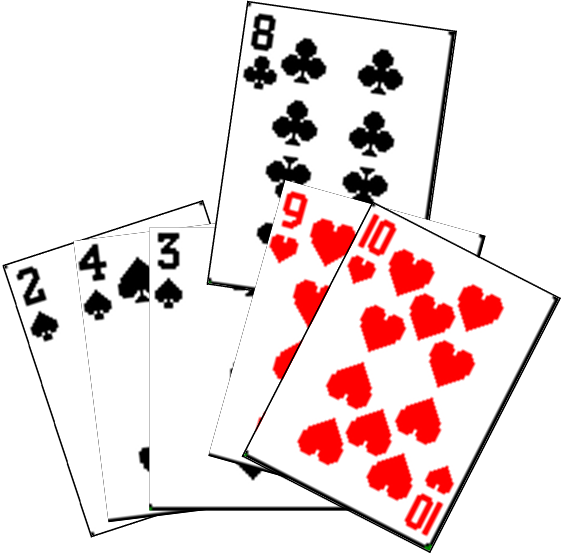
\includegraphics[scale=0.5]{img/card-deck}
  \caption{将草花8插入到一手牌中}
  \label{fig:hand-of-cards}
\end{figure}

\begin{algorithmic}[1]
\Function{Sort}{$A$}
  \State $S \gets$ NIL
  \For{each $a \in A$}
    \State \Call{Insert}{$a, S$}
  \EndFor
  \State \Return $S$
\EndFunction
\end{algorithmic}

这一实现将排序的结果存储在新数组$S$中,也可以复用原数组的空间进行就地排序:

\begin{algorithmic}[1]
\Function{Sort}{$A$}
  \For{$i \gets 2$ to $|A|$}
    \State ordered insert $A[i]$ to $A[1...(i-1)]$
  \EndFor
\EndFunction
\end{algorithmic}

其中索引$i$的范围是从1到$n = |A|$。只含有一个元素的子数组$[A[1]]$是已序的,因此我们从第二个元素开始插入。当处理第$i$个元素时,所有$i$之前的元素是已序的。我们不断将未排序的元素插入,如图\ref{fig:in-place-isort}所示。

\begin{figure}[htbp]
  \centering
  \includegraphics[scale=0.8]{img/in-place-sort}
  \caption{不断将元素插入已序部分}
  \label{fig:in-place-isort}
\end{figure}

\section{插入}
\index{插入排序!插入}

第一章给出了列表的插入算法。对于数组,也可以通过逐一检查找到插入位置。检查可以从左向右或者从右向左进行。下面的实现是从右向左进行检查的:

\begin{algorithmic}[1]
\Function{Sort}{$A$}
  \For{$i \gets 2$ to $|A|$}
    \Comment{Insert $A[i]$ to $A[1...(i-1)]$}
    \State $x \gets A[i]$ \Comment{将$A[i]$保存到$x$}
    \State $j \gets i-1$
    \While{$j > 0$ and $x < A[j]$ }
      \State $A[j+1] \gets A[j]$
      \State $j \gets j - 1$
    \EndWhile
    \State $A[j+1] \gets x$
  \EndFor
\EndFunction
\end{algorithmic}

由于数组是连续存储的,在某一位置插入元素是一个代价较高的操作。若在第$i$个位置插入元素$x$,需要把$i$后面的所有元素(包括$A[i+1]$、$A[i+2]$……)都向右移动一个位置。将第$i$个位置空出以放入$x$。如图\ref{fig:array-shift}所示。

\begin{figure}[htbp]
  \centering
  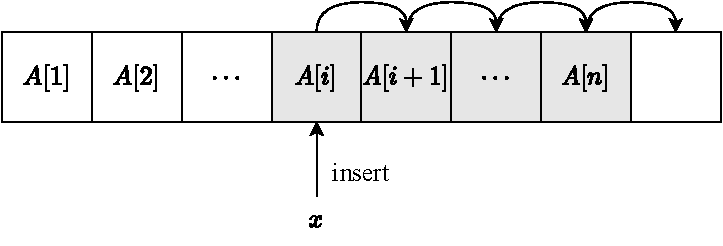
\includegraphics[scale=0.7]{img/array-shift}
  \caption{将元素$x$插入数组$A$中的第$i$个位置}
  \label{fig:array-shift}
\end{figure}

数组的长度为$n$,若比较$x$和前$i$个元素后,定位到了插入位置。接下来需要将剩余的$n - i + 1$的元素向后移动,再将$x$放入第$i$个位置。整体上看,我们相当于从左向右遍历了整个数组。另一方面,如果从右向左处理,则需要检查$n - i + 1$个元素,并执行相同数量的移动操作。我们也可以定义一个单独的\textproc{Insert}()函数,并在循环中调用。无论是从左向右或从右向左处理,插入操作都需要线性时间,因此插入排序的总体复杂度为$O(n^2)$,其中$n$是元素的个数。

\begin{Exercise}
\Question{实现从左向右处理的插入操作。}
\Question{定义单独的插入函数以实现插入排序。}
\end{Exercise}

\section{二分查找}
\index{插入排序!二分查找}

在玩扑克牌的时候,人们并不是逐一比较找到插入位置的。我们之所以能快速定位,是因为手中的牌在任何时刻都是已序的。二分查找是一种在已序序列中快速定位的方法。

\begin{algorithmic}[1]
\Function{Sort}{$A$}
  \For{$i \gets 2$ to $|A|$}
    \State $x \gets A[i]$
    \State $p \gets $ \Call{Binary-Search}{$x, A[1...(i-1)]$}
    \For{$j \gets i$ down to $p$}
      \State $A[j] \gets A[j-1]$
    \EndFor
    \State $A[p] \gets x$
  \EndFor
\EndFunction
\end{algorithmic}

二分查找时,数组中的片断$A[1...(i-1)]$是有序的。不失一般性,设其为单调增(可以定义抽象的$\leq$)。我们需要找到一个位置$j$使得$A[j-1] \leq x \leq A[j]$。我们先用$x$和中间位置的元素$A[m]$比较,其中$m = \lfloor \dfrac{i}{2} \rfloor$。如果$x < A[m]$,则递归地在前一半序列中二分查找;否则查找后一半序列。由于每次都排除掉一半元素,二分查找需要$O(\lg i)$的时间定位到插入点。

\begin{algorithmic}[1]
\Function{Binary-Search}{$x, A$}
  \State $l \gets 1, u \gets 1+|A|$
  \While{$l < u$}
    \State $m \gets \lfloor \dfrac{l+u}{2} \rfloor$
    \If{$A[m] = x$}
      \State \Return $m$ \Comment{重复元素}
    \ElsIf{$A[m] < x$}
      \State $l \gets m+1$
    \Else
      \State $u \gets m$
    \EndIf
  \EndWhile
  \State \Return $l$
\EndFunction
\end{algorithmic}

这一改进并不能提高插入排序的整体复杂度,结果仍然是$O(n^2)$。逐一比较的插入排序需要$O(n^2)$次比较和$O(n^2)$次移动;使用二分查找后,比较次数减少到了$O(n \lg n)$,但移动次数还是$O(n^2)$。

\begin{Exercise}
\Question{使用递归实现二分查找。}
\end{Exercise}

\section{列表}
\index{插入排序!列表插入排序}

二分查找将搜索时间降低到$O(n \lg n)$,但由于要依次移动数组中的元素,整体复杂度仍然是$O(n^2)$。另一方面,使用列表存储元素时,一旦获取了插入位置的引用,插入操作本身是常数时间的。在第一章中,我们定义了如下的列表插入排序算法:

\be
\begin{array}{rcl}
sort(\nil) & = & \nil \\
sort(x:xs) & = & insert(x, sort(xs)) \\
\end{array}
\ee

或使用$fold_l$的柯里化形式:

\be
sort = fold_l(insert, \nil)
\ee

由于需要遍历,列表的$insert$算法仍是线性时间的:

\be
\begin{array}{rcl}
insert(x,\ \nil) & = & [x] \\
insert(x,\ y : ys) & = & \begin{cases}
  x \leq y : & x : y : ys \\
  otherwise : & y : insert(x, ys) \\
  \end{cases}
\end{array}
\ee

\label{sec:list-index-array}
也可以不使用节点引用,而通过另一个索引数组来实现列表。对任何元素$A[i]$,$Next[i]$保存了$A[i]$之后下一个元素的索引。也就是说$A[Next[i]]$是$A[i]$的下一个元素。其中有两个特殊索引:对于列表的末尾元素$A[m]$,定义$Next[m] = -1$,表示其指向NIL;此外定义$Next[0]$指向列表的头部。利用索引数组,我们定义插入算法如下:

\begin{algorithmic}[1]
\Function{Insert}{$A, Next, i$}
  \State $j \gets 0$ \Comment{$Next[0]$指向表头}
  \While{$Next[j] \neq -1$ and $A[Next[j]] < A[i]$}
    \State $j \gets Next[j]$
  \EndWhile
  \State $Next[i] \gets Next[j]$
  \State $Next[j] \gets i$
\EndFunction
\Statex
\Function{Sort}{$A$}
  \State $n \gets |A|$
  \State $Next = [1, 2, ..., n, -1]$ \Comment{$n + 1$个索引}
  \For{$i \gets 1$ to $n$}
    \State \Call{Insert}{$A, Next, i$}
  \EndFor
  \State \Return $Next$
\EndFunction
\end{algorithmic}

使用列表,尽管在引用位置进行插入只需要常数时间,但必须遍历才能找到插入位置。整体仍需要$O(n^2)$次比较。与数组不同,列表不支持随机访问,不能利用二分查找提升定位速度。

\begin{Exercise}
\Question{使用索引数组,排序结果是一个重新排列的索引。给出一个方法,根据新的索引$Next$,重新排列数组$A$。}
\end{Exercise}

\section{二叉搜索树}
\index{插入排序!二叉搜索树}

我们遇到了一个困难境地:必须同时提高查找和插入的速度,仅提高其中之一仍然是$O(n^2)$的复杂度。一方面,我们希望用二分查找把比较次数降低到$O(\lg n)$;另一方面,需要改变数据结构,因为数组不支持在指定位置以常数时间插入元素。在第二章中,我们介绍了二叉搜索树。它天然就支持二分查找。一旦定位到插入位置,我们可以用常数时间插入新节点。

\begin{algorithmic}[1]
\Function{Sort}{$A$}
  \State $T \gets \nil$
  \For{each $x \in A$}
    \State $T \gets $ \Call{Insert-Tree}{$T, x$}
  \EndFor
  \State \Return \Call{To-List}{$T$}
\EndFunction
\end{algorithmic}

第二章给出了\textproc{Insert-Tree}()和\textproc{To-List}()的定义。平均情况下,树排序的复杂度为$O(n \lg n)$,其中$n$是元素的个数。这达到了基于比较的排序算法时间下限(\cite{Knuth-V3}第180-193页、\cite{CLRS}第167页)。但在最坏情况下,当树极度不平衡时,其性能会下降到$O(n^2)$。

\section{小结}
很多情况下,插入排序常作为第一个排序算法被介绍。它简单直观,但性能是平方级别的。插入排序不仅出现在教科书中,也出现在快速排序的工程实现中:在小数据集时回退到插入排序以抵消递归的代价。

\ifx\wholebook\relax \else
\begin{thebibliography}{99}

\bibitem{CLRS}
Thomas H. Cormen, Charles E. Leiserson, Ronald L. Rivest and Clifford Stein.
``Introduction to Algorithms, Second Edition''. (《算法导论》中文版)ISBN:0262032937. The MIT Press. 2001

\bibitem{Knuth-V3}
Donald E. Knuth. ``The Art of Computer Programming, Volume 3: Sorting and Searching (2nd Edition)''. Addison-Wesley Professional; 2 edition (May 4, 1998) ISBN-10: 0201896850 ISBN-13: 978-0201896855

\end{thebibliography}

\end{document}
\fi
